\documentclass{article}
\usepackage[usenames,dvipsnames,svgnames]{xcolor}
\usepackage[utf8]{inputenc}
\usepackage{algpseudocode}
\usepackage{amsfonts}
\usepackage{amsmath}
\usepackage{amssymb}
\usepackage{amsthm}
\usepackage{algorithm}
\usepackage{tikz}
\usepackage{subcaption}
\usepackage{fancyvrb}
\usepackage{bm}
\usepackage{textcomp}
\usepackage{listings}
\usepackage{todonotes}
\usepackage{mathtools} % long right arrow
\usepackage{proof} % for infer
\usepackage{setspace} % set line spacing
\usepackage{amsthm}

\newtheorem{theorem}{Theorem}[section]
\newtheorem{corollary}{Corollary}[theorem]
\newtheorem{lemma}[theorem]{Lemma}
\newtheorem{definition}{Definition}[section]

\newcommand{\code}[1]{\texttt{\small{\textbf{#1}}}}
\newcommand{\reals}[0]{\mathbb{R}}
\newcommand{\naturals}[0]{\mathbb{N}}
\newcommand{\integers}[0]{\mathbb{Z}}
\newcommand{\rationals}[0]{\mathbb{Q}}
\newcommand\doubleplus{\mathbin{+\mkern-5mu+}}
\newcommand{\concat}[0]{\doubleplus}
\newcommand{\dom}[1]{\mbox{dom}{~#1}}
\newcommand{\emptyassignment}[0]{\epsilon}
\newcommand{\gen}[0]{\mbox{\scriptsize gen}}
\newcommand{\force}[0]{\mbox{\scriptsize force}}
\newcommand{\fix}[0]{\mbox{\scriptsize fix}}
\newcommand{\free}[0]{\mbox{\scriptsize free}}
\newcommand{\contained}[0]{\sqsubseteq}
\newcommand{\auxassign}[0]{\alpha}
\newcommand{\aux}[0]{\mbox{\scriptsize aux}}

% coordinates for tikz address schematics
\newcommand{\innerll}[0]{(0.25 + 0.625, 0.625)}
\newcommand{\innerlr}[0]{(0.25 + 0.625 + 0.5, 0.625)}
\newcommand{\innerur}[0]{(0.25 + 0.625 + 0.5, 0.625 + 0.5)}
\newcommand{\innerul}[0]{(0.25 + 0.625, 0.625 + 0.5)}
\newcommand{\outerll}[0]{(0.25, 0)}
\newcommand{\outerlr}[0]{(0.25 + 1.75, 0)}
\newcommand{\outerur}[0]{(0.25 + 1.75, 1.75)}
\newcommand{\outerul}[0]{(0.25, 1.75)}
\newcommand{\all}[0]{(0, 0)}
\newcommand{\alr}[0]{(2, 0)}
\newcommand{\aur}[0]{(2, 2)}
\newcommand{\aul}[0]{(0, 2)}
\newcommand{\bll}[0]{(0.25, -0.25)}
\newcommand{\blr}[0]{(2.25, -0.25)}
\newcommand{\bur}[0]{(2.25, 1.75)}
\newcommand{\bul}[0]{(0.25, 1.75)}

\title{Gen Semantics}
\author{Marco Cusumano-Towner}

\begin{document}

\maketitle

\section{Assignments}
A \emph{assignment} is a finite map from a countable set of \emph{addresses} to \emph{values}, which for simplicity, we assume are elements of some finite set $V$.
The `set of addresses' in an assignment $t$ is its domain $\dom{t}$.
For assignments $s$ and $t$ with disjoint domains $\dom{s}$ and $\dom{t}$, let $u = s \concat t$ denote the assignment $u$ with $\dom{u} = \dom{s} \cup \dom{t}$ and $u(a) = s(a)$ for $a \in \dom{s}$ and $u(a) = t(a)$ for $a \in \dom{t}$.
For two assignments $s$ and $t$, let $s \contained t$ denote the relation that $\dom{s} \subseteq \dom{t}$ and that $s(a) = t(a)$ for all $a \in \dom{s}$ ($s$ is a restriction of $t$).
Let $t|_S$ denote the restriction of a assignment $t$ to a set $S$ of addresses, so that $\dom{t|_S} = \dom{t} \cap S$.
Let $\emptyassignment$ denote the empty assignment ($\dom \emptyassignment = \varnothing$).

\section{Probabilistic Module}
A \emph{probabilistic module} is a tuple $(X, P, \theta, f, U^{\gen}, Q^{\gen}, Q^{\fix}, Q^{\free})$.
Each of these elements is explained below.

\paragraph{Input type}
$X$ is the set of valid \emph{inputs} to the module, denoted $x \in X$.

\paragraph{Generative distribution}
The \emph{generative distribution} of a probabilistic module for input $x \in X$ is denoted $P_x$, where $P_x(t) \ge 0$ where $t$ is a assignment and $\sum_t P_x(t) = 1$.
Let $T_x := \{t : P_x(t) > 0 \}$ denote the set of \emph{possible assignments} for input $x \in X$.
We require that $P$ satisfies the following \emph{well-behaved addresses property}:
For all $x \in X$ and all $s, t \in T_x$, if $\dom{s} \ne \dom{t}$ then $\exists a \in \dom{s} \cap \dom{t}$ such that $s(a) \ne t(a)$.
In words, different address sets for the same arguments $x$ must be explained by different value{s} for some shared address(es).

\paragraph{Output function}
The \emph{output function} $f : \{(x, t) : x \in X, t \in T_x\} \to Y$ defines the \emph{output value} $y \in Y$ given the inputs $x$ and an assignment.

\paragraph{Static parameters}
The generative distribution may be parametrized by trainable \emph{static parameters} $\theta$, in which case $P_x(t)$ is replaced with $P_{x,\theta}(t)$.
See \code{backprop\_params} below.

% TODO all of the methods will accept arbitary configuration, which is
% recursively dispatched throughout the call hierarchy during calls to methods.
% the address selection is one example type of configuration used to configure
% free_update.

%%%%%%%%%%%%%%
%% generate %%
%%%%%%%%%%%%%%

\paragraph{Generate Method (\code{generate})}
For each $x \in X$, $U^{gen}_x$ is a set of assignments, called \emph{valid generation constraints}, such that for each $u \in U^{\gen}_x$ there exists some $t \in T_x$ where $u \contained t$.
$U^{\gen}_x$ need not include all such $u$ (i.e. $U^{\gen}_x$ is not necessarily the set of all projections of all assignments in $T_x$).
We require that $\emptyassignment \in U^{\gen}_x$ and that $T_x \subseteq U^{\gen}_x$.
For each $x \in X$ and $u \in U^{\gen}_x$, $Q^{\gen}_{x,u}$ is a probability distribution on assignments $s$ such that $Q^{\gen}_{x,u}(s) > 0$ if and only if $t = s \concat u$ for some $t \in T_x$.
The distribution is normalized ($\sum_s Q^{\gen}_{x,u}(s) = 1$).
Given $x \in X$ and $u \in U^{\gen}_x$, sample $s \sim Q^{\gen}_{x,u}(\cdot)$, and return $t = s \concat u$ and a weight $P_x(t) / Q^{\gen}_{x,u}(s)$.
Also return $y = f(x, t)$.

%% generate address schematic %%
\begin{figure}[t]
\centering
% dom t
\begin{subfigure}[b]{0.3\textwidth}
\centering
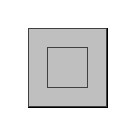
\begin{tikzpicture}
\draw (0, 0) rectangle (1, 1);
\draw (0.25, 0.25) rectangle (0.75, 0.75);
\filldraw [gray, fill opacity=0.5, draw opacity=0.0] (0, 0) -- (0, 1) -- (1, 1) -- (1, 0);
\end{tikzpicture}
\caption{$\dom{t}$}
\end{subfigure}%
% dom u
\begin{subfigure}[b]{0.3\textwidth}
\centering
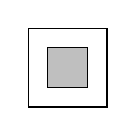
\begin{tikzpicture}
\draw (0, 0) rectangle (1, 1);
\draw (0.25, 0.25) rectangle (0.75, 0.75);
\filldraw [gray, fill opacity=0.5, draw opacity=0.0] (0.25, 0.25) -- (0.25, 0.75) -- (0.75, 0.75) -- (0.75, 0.25);
\end{tikzpicture}
\caption{$\dom{u}$}
\end{subfigure}
% dom s
\begin{subfigure}[b]{0.3\textwidth}
\centering
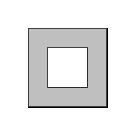
\begin{tikzpicture}
\draw (0, 0) rectangle (1, 1);
\draw (0.25, 0.25) rectangle (0.75, 0.75);
\filldraw [gray, fill opacity=0.5, draw opacity=0.0] (0, 0) -- (1, 0) -- (1, 1) -- (0, 1) (0.25, 0.25) -- (0.25, 0.75) -- (0.75, 0.75) -- (0.75, 0.25);
\end{tikzpicture}
\caption{$\dom{s}$}
\end{subfigure}
\caption{Schematic showing addresses of assignments involved in \code{generate}}
\end{figure}

\paragraph{Propose Method (\code{propose})}
Given $x \in X$, and a set of addresses $A$ such that for all $t \in T_x$, $t|_A \in U^{\gen}_x$, sample $t \sim P_x(\cdot)$, then decompose $t = u \concat s$ where $u = t|_A$, and return $u$ and the weight $P_x(t) / Q^{\gen}_{x,u}(s)$.
Also return $y = f(x, t)$.


%%%%%%%%%%%%%%%%%%
%% force update %%
%%%%%%%%%%%%%%%%%%

\paragraph{Force Update Method (\code{force\_update})}
For $x, x' \in X$, and $t \in T_x$, let $U^{\force}_{x,x',t}$ denote the set of assignments $u$ such that there exists $t' \in T_{x'}$ where $u \contained t'$ and $\{ a: t(a) \ne t'(a)\} \subseteq \dom{u}$, and $\dom{t'} \setminus \dom{t} \subseteq \dom{u}$.
That is, $u$ contains values for at least all addresses that differ between $t$ and $t'$, and all addresses in $t'$ that are not in $t$.
Return $t'$ (see Lemma~\ref{lemma:force-update-unique} for uniqueness of $t'$), and the weight $p(t'; x') / p(t; x)$ and $y = f(x', t')$.
Also return the \emph{discard assignment} $v$ given by $v(a) = t(a)$ for $a \in (\dom{t'} \setminus \dom{t}) \cup (\dom{t} \cap \dom{u})$.

\begin{lemma} \label{lemma:force-update-unique}
For any such $x, x', t, u$, the assignment $t'$ is unique.
\end{lemma}
\begin{proof}
Suppose there exists $t'_1 \ne t'_2$ such that $u \contained t'_1$ and $u \contained t'_2$ and such that $\dom{u} \supseteq \{a : t(a) \ne t'_1(a) \lor t(a) \ne t'_2(a)\} \cup ((\dom{t'_1} \cup \dom{t'_2}) \setminus \dom{t})$.
If $\dom{t'_1} = \dom{t'_2}$ then there must be an address $b$ such that $t'_1(b) \ne t(b)$ or $t'_2(b) \ne t(b)$, which implies $b \in \dom{u}$, which implies $t'_1(b) = t'_2(b) = u(b)$, which is a contradiction.
If $\dom{t'_1} \ne \dom{t'_2}$, then by the well-behaved address property, there must be an address $b$ such that $t'_1(b) \ne t'_2(b)$, which implies $b \in \dom{u}$, which implies $t'_1(b) = t'_2(b) = u(b)$, which is a contradiction.
\end{proof}

%% force update address schematic %%
\begin{figure}[t]
\centering
% dom t
\begin{subfigure}[b]{0.2\textwidth}
\centering
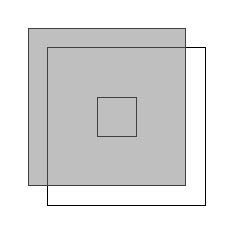
\begin{tikzpicture}
\draw \all{} rectangle \aur{};
\draw \bll{} rectangle \bur{};
\draw \innerll{} rectangle \innerur{};
\filldraw [gray, fill opacity=0.5, draw opacity=0.0] \all{} -- \alr{} -- \aur{} -- \aul{};
\end{tikzpicture}
\caption{$\dom{t}$}
\end{subfigure}%
% dom t'
\begin{subfigure}[b]{0.2\textwidth}
\centering
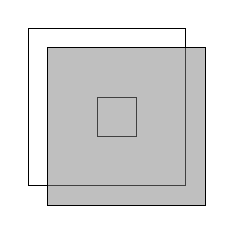
\begin{tikzpicture}
\draw \all{} rectangle \aur{};
\draw \bll{} rectangle \bur{};
\draw \innerll{} rectangle \innerur{};
\filldraw [gray, fill opacity=0.5, draw opacity=0.0] \bll{} -- \blr{} -- \bur{} -- \bul{};
\end{tikzpicture}
\caption{$\dom{t'}$}
\end{subfigure}%
% dom u
\begin{subfigure}[b]{0.2\textwidth}
\centering
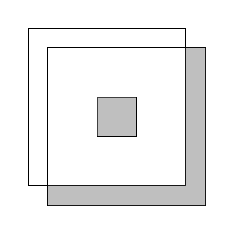
\begin{tikzpicture}
\draw \all{} rectangle \aur{};
\draw \bll{} rectangle \bur{};
\draw \innerll{} rectangle \innerur{};
\filldraw [gray, fill opacity=0.5, draw opacity=0.0] \innerll{} -- \innerlr{} -- \innerur{} -- \innerul{};
\filldraw [gray, fill opacity=0.5, draw opacity=0.0] \outerll{} -- \outerlr{} -- \outerur{} -- \bur{} -- \blr{} -- \bll{} -- \outerll{};
\end{tikzpicture}
\caption{$\dom{u}$}
\end{subfigure}%
% dom v
\begin{subfigure}[b]{0.2\textwidth}
\centering
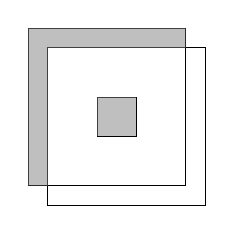
\begin{tikzpicture}
\draw \all{} rectangle \aur{};
\draw \bll{} rectangle \bur{};
\draw \innerll{} rectangle \innerur{};
\filldraw [gray, fill opacity=0.5, draw opacity=0.0] \innerll{} -- \innerlr{} -- \innerur{} -- \innerul{};
\filldraw [gray, fill opacity=0.5, draw opacity=0.0] \outerll{} -- \outerul{} -- \outerur{} -- \aur{} -- \aul{} -- \all{} -- \outerll{};
\end{tikzpicture}
\caption{$\dom{v}$}
\end{subfigure}%
% dom r
\begin{subfigure}[b]{0.2\textwidth}
\centering
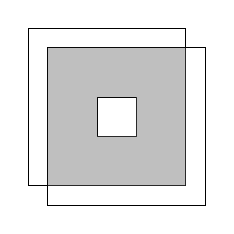
\begin{tikzpicture}
\draw \all{} rectangle \aur{};
\draw \bll{} rectangle \bur{};
\draw \innerll{} rectangle \innerur{};
\filldraw [gray, fill opacity=0.5, draw opacity=0.0] \outerll{} -- \outerlr{} -- \outerur{} -- \outerul{} \innerll{} -- \innerul{} -- \innerur{} -- \innerlr{};
\end{tikzpicture}
\caption{$\dom{r}$}
\end{subfigure}
\caption{Schematic showing addresses of assignments involved in \code{force\_update}}
\end{figure}


%%%%%%%%%%%%%%%%
%% fix update %%
%%%%%%%%%%%%%%%%

\paragraph{Fix Update Method (\code{fix\_update})}
For $x, x' \in X$ and $t \in T_x$, let $U^{\fix}_{x,x',t}$ denote the set of assignments $u$ such that $\dom{u} \subseteq \dom{t}$ and such that there exists assignments $s$ and $r$ with $\dom{s} \cap \dom{t} = \varnothing$, $\dom{r} \subseteq \dom{t}$, $\dom{r} \cap \dom{u} = \varnothing$ where $u \concat s \concat r \in T_{x'}$.
For each $x, x' \in X$, $t \in T_x$, and $u \in U^{\fix}_{x,x',t}$, there is a probability distribution on assignments $s$, denoted $Q^{\fix}_{x,x',t,u}(s)$, such that $Q^{\fix}_{x,x',t,u}(s) > 0$ if and only if there exists a assignment $r$ with $\dom{r} \subseteq \dom{t}$ and $\dom{r} \cap \dom{u} = \varnothing$ where $t' = u \concat s \concat r \in T_{x'}$.

\begin{lemma} \label{lemma:fix-update-unique}
For any such $x, x', t, u, s$, the assignments $r$ and $t'$ are unique.
\end{lemma}
\begin{proof}
\end{proof}

Given $x, x' \in X, t \in T_x, u \in U^{\fix}_{x,x',t}$, sample $s \sim Q^{\fix}_{x,x',t,u}(\cdot)$ and return $t' = u \concat s \concat r$, the \emph{discard assignment} $v$ where $v(a) = t(a)$ for $a \in \dom{u}$, and the weight:
\[
\frac{p(t'; x')}{p(t; x)} \frac{Q^{\fix}_{x',x,t',v}(s')}{Q^{\fix}_{x,x',t,u}(s)}
\]
where $s' = t|_{\dom{t} \setminus \dom{t'}}$ contains the part of $t$ that was \emph{deleted}.
Also return $y = f(x', t')$.

\begin{lemma} \label{lemma:fix-update-reverse}
If $x, x' \in X, t \in T_x, u \in U^{\fix}_{x, x', t}$, and $s$ where $Q^{\fix}_{x,x',t,u}(s) > 0$, $v \in U^{\fix}_{x',x,t'}$ and $Q^{\fix}_{x',x,t'}(s') > 0$, then $v \concat s' \concat r = t$.
\end{lemma}
\begin{proof}
\end{proof}

%% fix update address schematic %%
\begin{figure}[t]
\centering
% dom t
\begin{subfigure}[b]{0.3\textwidth}
\centering
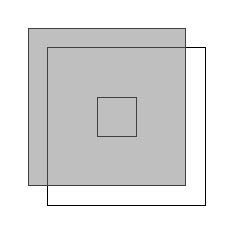
\begin{tikzpicture}
\draw \all{} rectangle \aur{};
\draw \bll{} rectangle \bur{};
\draw \innerll{} rectangle \innerur{};
\filldraw [gray, fill opacity=0.5, draw opacity=0.0] \all{} -- \alr{} -- \aur{} -- \aul{};
\end{tikzpicture}
\caption{$\dom{t}$}
\end{subfigure}%
% dom t'
\begin{subfigure}[b]{0.3\textwidth}
\centering
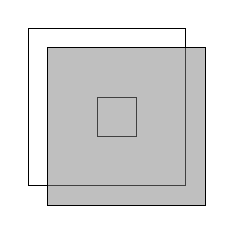
\begin{tikzpicture}
\draw \all{} rectangle \aur{};
\draw \bll{} rectangle \bur{};
\draw \innerll{} rectangle \innerur{};
\filldraw [gray, fill opacity=0.5, draw opacity=0.0] \bll{} -- \blr{} -- \bur{} -- \bul{};
\end{tikzpicture}
\caption{$\dom{t'}$}
\end{subfigure}%
% dom u = dom v
\begin{subfigure}[b]{0.3\textwidth}
\centering
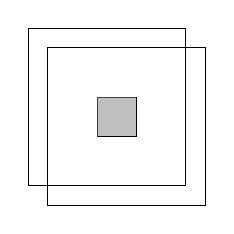
\begin{tikzpicture}
\draw \all{} rectangle \aur{};
\draw \bll{} rectangle \bur{};
\draw \innerll{} rectangle \innerur{};
\filldraw [gray, fill opacity=0.5, draw opacity=0.0] \innerll{} -- \innerlr{} -- \innerur{} -- \innerul{};
\end{tikzpicture}
\caption{$\dom{u} = \dom{v}$}
\end{subfigure}\\
% dom s
\begin{subfigure}[b]{0.3\textwidth}
\centering
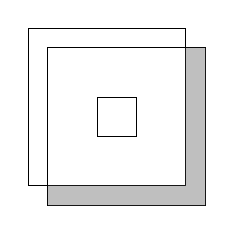
\begin{tikzpicture}
\draw \all{} rectangle \aur{};
\draw \bll{} rectangle \bur{};
\draw \innerll{} rectangle \innerur{};
\filldraw [gray, fill opacity=0.5, draw opacity=0.0] \outerll{} -- \outerlr{} -- \outerur{} -- \bur{} -- \blr{} -- \bll{} -- \outerll{};
\end{tikzpicture}
\caption{$\dom{s}$}
\end{subfigure}%
% dom s'
\begin{subfigure}[b]{0.3\textwidth}
\centering
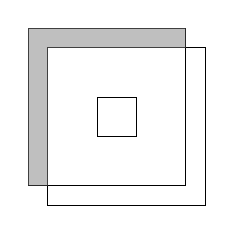
\begin{tikzpicture}
\draw \all{} rectangle \aur{};
\draw \bll{} rectangle \bur{};
\draw \innerll{} rectangle \innerur{};
\filldraw [gray, fill opacity=0.5, draw opacity=0.0] \outerll{} -- \outerul{} -- \outerur{} -- \aur{} -- \aul{} -- \all{} -- \outerll{};
\end{tikzpicture}
\caption{$\dom{s'}$}
\end{subfigure}%
% dom r
\begin{subfigure}[b]{0.3\textwidth}
\centering
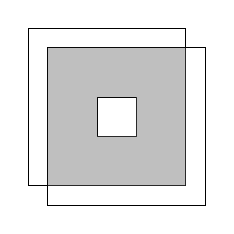
\begin{tikzpicture}
\draw \all{} rectangle \aur{};
\draw \bll{} rectangle \bur{};
\draw \innerll{} rectangle \innerur{};
\filldraw [gray, fill opacity=0.5, draw opacity=0.0] \outerll{} -- \outerlr{} -- \outerur{} -- \outerul{} \innerll{} -- \innerul{} -- \innerur{} -- \innerlr{};
\end{tikzpicture}
\caption{$\dom{r}$}
\end{subfigure}
\caption{Schematic showing addresses of assignments involved in \code{fix\_update}}
\end{figure}


%%%%%%%%%%%%%%%%%
%% free update %%
%%%%%%%%%%%%%%%%%

\paragraph{Free Update Method (\code{free\_update})}
Given $x, x' \in X$, and $t \in T_x$, $Q^{\free}_{t,x,x'}(t')$ is a distribution on assignments such that $Q^{\free}_{t,x,x'}(t') > 0$ implies $t' \in T_{x'}$, and such that $Q^{\free}_{t,x,x'}(t') > 0$ implies $Q^{\free}_{t',x',x}(t) > 0$.
Sample $t' \sim Q^{\free}_{t,x,x'}(\cdot)$ and return $t'$, and a weight:
\[
    \frac{p(t'; x')}{p(t; x)} \frac{Q^{\free}_{t',x',x}(t)}{Q^{\free}_{t,x,x'}(t')}
\]
Also return $y' = f(x', t')$.
Note that `regenerate', where we provide a set of addresses that should be resimulated, is an example of this.

\paragraph{Backpropagate to Parameters Method (\code{backprop\_params})}
Given $x \in X$ and $t \in T_x$, and $\nabla_y J$, return $\nabla_x (J + \log p(t; x))$ and $\nabla_{\theta} (J + \log p(t; x))$.

% \paragraph{Backpropagate to Trace (\code{backprop\_assignment})}
% TODO doesn't make sense if values come from a discrete set

Each probabilistic module may also possess an indexed collection of families of distributions for use in \code{generate} and \code{update}.
Probabilistic modules may also have update procedures that make arbitrary changes to their assignment, and return the appropriate weight.
These two features are not yet implemented.

\section{Auxiliary Randomness}
In this section, we generalize the above interface to support \emph{auxiliary random choices}, which permit encapsulation of internal randomness within a probabilistic module.
Unlike traced assignments ($t$), auxiliary assignments (denoted $\auxassign$) are not exposed as user-readable.
We replace the generative distribution $P_x(t)$ with a distribution $P_x(\auxassign, t)$ where $\auxassign$ is an assignment with $\dom{\auxassign} \cap \dom{t} = \varnothing$ for all $\auxassign, t$.
The marginal distribution of $P_x(\auxassign, t)$ is $P_x(t) := \sum_{\auxassign} P_x(\auxassign, t)$.
We define $T_x$ as $\{t : P_x(t) > 0\}$.
We replace the function $f$ with $f : \{(x, \auxassign, t) : P_x(\auxassign, t) > 0 \} \to Y$ (i.e. the output value can depend on the auxiliary randomness).
The module tuple is extended to include a family of distributions on the untraced assignments, denoted $Q^{\aux}_{x,t}(\auxassign)$, where $Q^{\aux}_{x,t}(\auxassign) > 0$ if and only if $P_x(\auxassign, t) > 0$.
Each of the methods above is adjusted as follows:

\paragraph{Generate Method (\code{generate})}
In addition to sampling $s \sim Q^{\gen}_{x,u}(\cdot)$, we also sample $\auxassign \sim Q^{\aux}_{x,t}(\cdot)$.
We return the weight $P_x(\auxassign, t) / (Q^{\gen}_{x,u}(s) Q^{\aux}_{x,t}(\auxassign))$
We return $t$ and $\auxassign$.

\paragraph{Propose Method (\code{propose})}
Instead of sampling $t \sim P_x(\cdot)$, we sample jointly $\auxassign, t \sim P_x(\cdot, \cdot)$.
We return $t$ and $\auxassign$.
We return the weight $P_x(\auxassign, t) / (Q^{\gen}_{x,u}(s) Q^{\aux}_{x,t}(\auxassign))$

\paragraph{Force Update Method (\code{force\_update})}
In addition to $x, x', t, u$, we accept $\auxassign$ such that $P_x(\auxassign, t) > 0$.
After computing $t'$, we sample $\auxassign' \sim Q^{\aux}_{x',t'}(\cdot)$.
We return the weight:
\[
\left( \frac{P_{x'}(\auxassign', t')}{Q^{\aux}_{x',t'}(\auxassign')} \right)
\bigg/
\left( \frac{P_x(\auxassign, t)}{Q^{\aux}_{x,t}(\auxassign)} \right)
\]

\paragraph{Fix Update Method (\code{fix\_update})}
In addition to $x, x', t, u$, we accept $\auxassign$ such that $P_x(\auxassign, t) > 0$.
After sampling $s$ and computing $t'$, we sample $\auxassign' \sim Q^{\aux}_{x',t'}(\cdot)$.
We return $(t, \auxassign)$ in addition to the weight:
\[
\left( \frac{P_{x'}(\auxassign', t')}{Q^{\fix}_{x,x',t,u}(s) Q^{\aux}_{x',t'}(\auxassign')} \right)
\bigg/
\left( \frac{P_x(\auxassign, t)}{Q^{\fix}_{x',x,t',v}(s') Q^{\aux}_{x,t}(\auxassign)} \right)
\]

\paragraph{Free Update Method (\code{free\_update})}
In addition to $x, x', t$, we accept $\auxassign$ such that $P_x(\auxassign, t) > 0$.
After sampling $t'$, we sample $\auxassign' \sim Q^{\aux}_{x',t'}(\cdot)$.
We return $(t, \auxassign)$ in addition to the weight:
\[
\left( \frac{P_{x'}(\auxassign', t')}{Q^{\free}_{x,x',t}(t') Q^{\aux}_{x',t'}(\auxassign')} \right)
\bigg/
\left( \frac{P_x(\auxassign, t)}{Q^{\free}_{x',x,t'}(t') Q^{\aux}_{x,t}(\auxassign)} \right)
\]

\subsection{Untraced Auxiliary Assignments}
Because auxiliary assignments are not exposed as user-readable, modules may choose to make use of the following optimization.
Note that auxiliary assignments are only ever referenced as part of ratios of the form $P_x(t) / Q^{\aux}_{x,t}(\auxassign)$.
Therefore, modules may compactly summarize the sufficient information about the auxiliary randomness in the form of this ratio.

\section{Generative Functions}
Generative functions are one type of probabilistic module, in which the generative function $P_x$ is defined as a Julia function extended with probabilistic semantics.
This section informally describes how generative functions implement each of the components of the probabilitsic module interface.

\paragraph{Input type}
The input type $X$ is the Julia type of the arguments to the function.

\paragraph{Generative Distribution}
The assignments $t$ generated by a generative function have a hierarchical structure.
Each \emph{address key} used with the \code{@addr} keyword is either a \emph{primitive address}, which is the address of a single random choice sampled from a probability distribution with known probability mass function, or a \emph{namespace}, under which the assignment of a called probabilistic module is generated.
The generative distribution $P_x(t)$ is defined by the product of probabilities of primitive addresses taking given values, with the probability of assignments to namespaces determined by the called probabilistic modules.
Auxiliary randomness $\auxassign$ consists of random choices that are not annotated with \code{@addr}.
For $Q^{\aux}_{x,t}$ we use forward evaluation, so that $P_x(t) / Q^{\aux}_{x,t}(\auxassign)$ is typically computed simply as a product of probabilities that skips over factors for the auxiliary addresses, due to cancellation of factors.

\paragraph{Output function}
The output function maps a terminating state of the function to the output value $y$, where the state of the function is a (deterministic) function of $x$, $\auxassign$, and $t$.

\paragraph{Generate Method (\code{generate})}
For $Q^{\gen}_{x,u}$ we use forward evaluation for primitive addresses, so that the weight is computed as a product of probabilities in $\dom{u}$ only, due to cancellation of factors for addresses in $\dom{s}$.
For addresses in namespaces we recursively invoke \code{generate}.

\paragraph{Propose Method (\code{propose})}
See `Generative Method'.

\paragraph{Force Update Method (\code{force\_update})}
For addresses in namespaces we recursively invoke \code{force\_update}.

\paragraph{Fix Update Method (\code{fix\_update})}
For $Q^{\fix}_{x,t}$ we use forward simulation of primitive addresses, and we for addresses in namespaces we recursively invoke \code{fix\_update}.

\paragraph{Free Update Method (\code{free\_update})}
% TODO accepts a set of addresses to resimulate... recursiely calls?

\subsection{Untraced Auxiliary Assignments}
Because auxiliary assignments are not exposed as user-readable, modules may choose to make use of the following optimization.
Note that auxiliary assignments are only ever referenced as part of ratios of the form $P_x(t) / Q^{\aux}_{x,t}(\auxassign)$.
Therefore, modules may compactly summarize the sufficient information about the auxiliary randomness in the form of this ratio.




\clearpage
\bibliographystyle{abbrv}
\bibliography{references}

\end{document}
